\documentclass[a4paper,12pt]{article}
\usepackage[utf8]{inputenc}
\usepackage[ngerman]{babel}
\usepackage{amsmath}
\usepackage{amssymb}
\usepackage{amsthm}
\usepackage{geometry}
\usepackage{graphicx}
\usepackage{booktabs}
\usepackage{float}
\usepackage[dvipsnames,svgnames]{xcolor}
\definecolor{deepblue}{RGB}{0,38,100}
\usepackage[
  colorlinks=true,
  linkcolor=deepblue,
  urlcolor=deepblue,
  citecolor=deepblue
]{hyperref}

\geometry{margin=2.5cm}

\theoremstyle{definition}
\newtheorem{definition}{Definition}
\newtheorem{beispiel}{Beispiel}
\newtheorem{satz}{Satz}
\newtheorem{lemma}{Lemma}
\newtheorem{korollar}{Korollar}
\newtheorem{beobachtung}{Beobachtung}

\title{Die au\ss ergewöhnliche Asymmetrie in der Reihendarstellung der
       Exponentialfunktion \\[0.5ex]
       \large Strukturelle Zerlegung, Komplexitätsunterschiede und
       parallele Berechnung}
\author{Stephan Epp}
\date{\today}

\begin{document}

\maketitle
\tableofcontents
\newpage

%% ─────────────────────────────────────────────────────────────────────────────
\section{Einführung}
%% ─────────────────────────────────────────────────────────────────────────────

Die Exponentialfunktion $e^x$ ist eine der fundamentalsten Funktionen der
Mathematik. Ihre Reihendarstellung erscheint auf den ersten Blick homogen und
symmetrisch. Bei genauerer Betrachtung offenbart sich jedoch eine tiefe
strukturelle Asymmetrie, die weitreichende Konsequenzen für das Verständnis der
Funktion hat.

Die zentrale Beobachtung dieser Arbeit ist: Die geraden Glieder der Reihe sind
strukturell einfacher als die ungeraden Glieder. Achsensymmetrie ist
fundamentaler als Punktsymmetrie. Diese Erkenntnis ermöglicht eine alternative
Berechnungsstrategie: Berechne die geraden Glieder direkt, berechne die gesamte
Funktion, und erhalte die ungeraden Glieder als Differenz.

Dieser Ansatz ist nicht nur mathematisch elegant, sondern spiegelt ein tieferes
Prinzip wider: Komplexe Strukturen lassen sich oft effizienter durch Subtraktion
einfacherer Komponenten von einem Ganzen gewinnen als durch direkte Konstruktion.

%% ─────────────────────────────────────────────────────────────────────────────
\section{Strukturelle Zerlegung der Exponentialfunktion}
%% ─────────────────────────────────────────────────────────────────────────────

\subsection{Die Reihendarstellung}

\begin{definition}[Exponentialfunktion]
Die Exponentialfunktion ist definiert durch ihre Taylorreihe:
\begin{align}
  e^x = \sum_{n=0}^{\infty} \frac{x^n}{n!}
      = 1 + x + \frac{x^2}{2!} + \frac{x^3}{3!} + \frac{x^4}{4!}
        + \frac{x^5}{5!} + \cdots
\end{align}
Diese Reihe konvergiert für alle $x \in \mathbb{R}$ absolut.
\end{definition}

Diese scheinbar homogene Struktur verbirgt eine fundamentale Dualität zwischen
geraden und ungeraden Gliedern.

\subsection{Zerlegung in symmetrische Komponenten}

\begin{definition}[Gerade und ungerade Komponenten]
Die Exponentialfunktion lässt sich eindeutig zerlegen in:
\begin{align}
  e^x = E(x) + U(x)
\end{align}
wobei die \textbf{gerade Komponente} definiert ist als:
\begin{align}
  E(x) = \sum_{n=0}^{\infty} \frac{x^{2n}}{(2n)!}
       = 1 + \frac{x^2}{2!} + \frac{x^4}{4!} + \frac{x^6}{6!} + \cdots
\end{align}
und die \textbf{ungerade Komponente} als:
\begin{align}
  U(x) = \sum_{n=0}^{\infty} \frac{x^{2n+1}}{(2n+1)!}
       = x + \frac{x^3}{3!} + \frac{x^5}{5!} + \frac{x^7}{7!} + \cdots
\end{align}
\end{definition}

\begin{satz}[Symmetrieeigenschaften der Komponenten]
Die geraden und ungeraden Komponenten besitzen fundamentale
Symmetrieeigenschaften:
\begin{enumerate}
  \item $E(x)$ ist eine \textbf{gerade Funktion}: $E(-x) = E(x)$
        (Achsensymmetrie)
  \item $U(x)$ ist eine \textbf{ungerade Funktion}: $U(-x) = -U(x)$
        (Punktsymmetrie)
\end{enumerate}
\end{satz}

\begin{proof}
Für die gerade Komponente gilt:
\begin{align}
  E(-x) = \sum_{n=0}^{\infty} \frac{(-x)^{2n}}{(2n)!}
        = \sum_{n=0}^{\infty} \frac{x^{2n}}{(2n)!} = E(x)
\end{align}
da $(-1)^{2n} = 1$ für alle $n \in \mathbb{N}_0$.

Für die ungerade Komponente gilt:
\begin{align}
  U(-x) = \sum_{n=0}^{\infty} \frac{(-x)^{2n+1}}{(2n+1)!}
        = -\sum_{n=0}^{\infty} \frac{x^{2n+1}}{(2n+1)!} = -U(x)
\end{align}
da $(-1)^{2n+1} = -1$ für alle $n \in \mathbb{N}_0$.
\end{proof}

\subsection{Verbindung zu hyperbolischen Funktionen}

\begin{satz}[Darstellung durch Hyperbelfunktionen]
Die geraden und ungeraden Komponenten sind gegeben durch:
\begin{align}
  E(x) &= \cosh(x) = \frac{e^x + e^{-x}}{2} \\
  U(x) &= \sinh(x) = \frac{e^x - e^{-x}}{2}
\end{align}
\end{satz}

\begin{proof}
Addition der Identitäten ergibt:
\begin{align}
  E(x) + U(x)
    = \frac{e^x + e^{-x}}{2} + \frac{e^x - e^{-x}}{2} = e^x
\end{align}
Subtraktion mit $e^{-x} = E(x) - U(x)$ bestätigt die Darstellung.
\end{proof}

%% ─────────────────────────────────────────────────────────────────────────────
\section{Die fundamentale Asymmetrie: Achsensymmetrie versus Punktsymmetrie}
%% ─────────────────────────────────────────────────────────────────────────────

\subsection{Strukturelle Komplexität}

\begin{beobachtung}[Einfachheit der geraden Glieder]
Achsensymmetrie ist strukturell einfacher als Punktsymmetrie:
\begin{itemize}
  \item[-] \textbf{Achsensymmetrie} ($E(-x) = E(x)$): Erfordert nur, dass das
           Vorzeichen von $x$ irrelevant ist
  \item[-] \textbf{Punktsymmetrie} ($U(-x) = -U(x)$): Erfordert zusätzlich
           Vorzeichenwechsel des Funktionswerts
\end{itemize}
\end{beobachtung}

\subsubsection{Algebraische Struktur}

Für die gerade Komponente gilt:
\begin{align}
  E(x) = 1 + \frac{x^2}{2!} + \frac{x^4}{4!} + \frac{x^6}{6!} + \cdots
\end{align}
Jedes Glied ist \textbf{nicht-negativ} für $x \in \mathbb{R}$, da
$x^{2n} \geq 0$ für alle $n \in \mathbb{N}_0$.

Für die ungerade Komponente gilt:
\begin{align}
  U(x) = x + \frac{x^3}{3!} + \frac{x^5}{5!} + \frac{x^7}{7!} + \cdots
\end{align}
Die Glieder wechseln das Vorzeichen abhängig vom Vorzeichen von $x$.
Dies erfordert zusätzliche Vorzeichenverwaltung.

\subsubsection{Berechnungskomplexität}

\begin{lemma}[Effizienz der Potenzberechnung]
Die Berechnung von $x^{2n}$ ist effizienter als die von $x^{2n+1}$:
\begin{itemize}
  \item[-] $x^{2n} = (x^2)^n$: Erst Quadrieren, dann $n$-fache Multiplikation
  \item[-] $x^{2n+1} = x \cdot x^{2n}$: Zusätzliche Multiplikation mit $x$
\end{itemize}
Für große $n$ ist der relative Unterschied gering, aber strukturell ist
$x^{2n}$ direkter zugänglich.
\end{lemma}

\subsection{Geometrische Interpretation}

\begin{beobachtung}[Spiegelung versus Rotation]
Geometrisch entsprechen die Symmetrien unterschiedlichen Transformationen:
\begin{itemize}
  \item[-] \textbf{Achsensymmetrie}: Spiegelung an der $y$-Achse
           (eine Operation)
  \item[-] \textbf{Punktsymmetrie}: Rotation um $180^\circ$ um den Ursprung
           (Komposition zweier Spiegelungen)
\end{itemize}
Punktsymmetrie ist damit eine Komposition zweier elementarer Operationen.
\end{beobachtung}

%% ─────────────────────────────────────────────────────────────────────────────
\section{Alternative Berechnungsstrategie}
%% ─────────────────────────────────────────────────────────────────────────────

\subsection{Die Differenzmethode}

\begin{satz}[Berechnung durch Differenzbildung]
Seien $e^x$ und $E(x)$ bekannt. Dann lässt sich die ungerade Komponente
berechnen als:
\begin{align}
  U(x) = e^x - E(x)
\end{align}
Dies vermeidet die direkte Summation der komplizierten ungeraden Glieder.
\end{satz}

\begin{proof}
Nach Definition gilt $e^x = E(x) + U(x)$, also $U(x) = e^x - E(x)$.
\end{proof}

\subsubsection{Praktische Umsetzung}

Der Algorithmus zur Berechnung von $U(x)$ lautet:
\begin{enumerate}
  \item Berechne $E(x) = \cosh(x)$ durch Summation der geraden Glieder
  \item Berechne $e^x$ durch die vollständige Reihe
  \item Setze $U(x) = e^x - E(x)$
\end{enumerate}

\subsection{Verallgemeinertes Prinzip}

\begin{korollar}[Zerlegungsprinzip]
Sei $f(x) = f_{\text{einfach}}(x) + f_{\text{kompliziert}}(x)$, wobei
$f_{\text{einfach}}$ strukturell einfacher ist. Dann gilt:
\begin{align}
  f_{\text{kompliziert}}(x) = f(x) - f_{\text{einfach}}(x)
\end{align}
vorausgesetzt, $f(x)$ ist direkt zugänglich.
\end{korollar}

Dies ist ein fundamentales Prinzip der numerischen Mathematik:
\textbf{Komplexe Strukturen durch Subtraktion einfacher Komponenten gewinnen}.

%% ─────────────────────────────────────────────────────────────────────────────
\section{Verbindung zur Euler-Formel}
%% ─────────────────────────────────────────────────────────────────────────────

\subsection{Komplexe Exponentialfunktion}

\begin{satz}[Euler-Formel]
Für $x \in \mathbb{R}$ gilt:
\begin{align}
  e^{ix} = \cos(x) + i\sin(x)
\end{align}
wobei $\cos(x)$ und $\sin(x)$ die gerade bzw.\ ungerade Komponente der
komplexen Exponentialfunktion darstellen.
\end{satz}

\begin{proof}
Setze $x$ durch $ix$ in der Reihendarstellung:
\begin{align}
  e^{ix} = \sum_{n=0}^{\infty} \frac{i^n x^n}{n!}
\end{align}
Trenne nach Potenzen von $i$:
\begin{align}
  e^{ix} = \sum_{n=0}^{\infty} \frac{i^{2n} x^{2n}}{(2n)!}
          + \sum_{n=0}^{\infty} \frac{i^{2n+1} x^{2n+1}}{(2n+1)!}
\end{align}
Mit $i^{2n} = (-1)^n$ und $i^{2n+1} = i(-1)^n$ folgt:
\begin{align}
  e^{ix} = \sum_{n=0}^{\infty} \frac{(-1)^n x^{2n}}{(2n)!}
          + i \sum_{n=0}^{\infty} \frac{(-1)^n x^{2n+1}}{(2n+1)!}
         = \cos(x) + i\sin(x)
\end{align}
\end{proof}

\subsection{Asymmetrie im Komplexen}

\begin{lemma}[Komplexe Symmetrie]
Für die komplexe Exponentialfunktion gilt:
\begin{align}
  \operatorname{Re}(e^{ix}) &= \cos(x) = \text{gerade Komponente} \\
  \operatorname{Im}(e^{ix}) &= \sin(x) = \text{ungerade Komponente}
\end{align}
\end{lemma}

\begin{beobachtung}[Strukturelle Parallelität]
Die Asymmetrie zwischen Real- und Imaginärteil spiegelt die Asymmetrie
zwischen geraden und ungeraden Gliedern:
\begin{itemize}
  \item[-] $\cos(x)$: Gerade Funktion, nur gerade Potenzen, beginnt mit
           konstantem Glied~1
  \item[-] $\sin(x)$: Ungerade Funktion, nur ungerade Potenzen, beginnt mit
           linearem Glied~$x$
\end{itemize}
Die Cosinus-Funktion ist fundamentaler als die Sinus-Funktion, analog zu
$E(x)$ versus $U(x)$.
\end{beobachtung}

%% ─────────────────────────────────────────────────────────────────────────────
\section{Konvergenzverhalten und numerische Aspekte}
%% ─────────────────────────────────────────────────────────────────────────────

\subsection{Konvergenzgeschwindigkeit}

\begin{satz}[Relative Konvergenz]
Für festes $x \in \mathbb{R}$ haben beide Teilreihen $E(x)$ und $U(x)$
identische Konvergenzgeschwindigkeit, da beide Teilmengen derselben absolut
konvergenten Reihe sind.
\end{satz}

\begin{proof}
Das Verhältnis aufeinanderfolgender Glieder ist:
\begin{align}
  \frac{a_{n+1}}{a_n} = \frac{|x|}{n+1} \to 0 \quad \text{für } n \to \infty
\end{align}
Sowohl für gerade als auch ungerade Teilreihen gilt dasselbe asymptotische
Verhalten.
\end{proof}

\subsection{Numerische Stabilität der Differenzmethode}

\begin{beobachtung}[Auslöschungseffekte]
Die Differenzbildung $U(x) = e^x - E(x)$ unterliegt für große $x$ der
Auslöschung:
\begin{itemize}
  \item[-] Für $x \gg 1$: $e^x \approx E(x) \approx \frac{e^x}{2}$
           (beide sehr groß), die Differenz verliert relative Präzision
  \item[-] Für $x$ klein: $E(x) \approx 1$, $U(x) \approx x$,
           keine Auslöschung
\end{itemize}
\end{beobachtung}

\begin{satz}[Optimaler Berechnungsbereich]
Die Differenzmethode ist numerisch stabil für $|x| < 1$. Für $|x| > 1$
sollte direkte Summation verwendet werden.
\end{satz}

\begin{beispiel}[Partielle Summen für $x=1$]
Exakte Werte: $E(1) = \cosh(1) \approx 1.5431$,
$U(1) = \sinh(1) \approx 1.1752$.

\begin{center}
\begin{tabular}{c|c|c|c|c}
  $N$ & $E_N(1)$ & $|E(1)-E_N(1)|$ & $U_N(1)$ & $|U(1)-U_N(1)|$ \\
  \hline
  0 & 1.0000 & 0.5431 & 1.0000 & 0.1752 \\
  1 & 1.5000 & 0.0431 & 1.1667 & 0.0085 \\
  2 & 1.5417 & 0.0014 & 1.1750 & 0.0002 \\
  3 & 1.5431 & 0.0000 & 1.1752 & 0.0000 \\
\end{tabular}
\end{center}
Beide Reihen konvergieren gleich schnell.
\end{beispiel}

%% ─────────────────────────────────────────────────────────────────────────────
\section{Parallele Berechnung der Exponentialfunktion}
%% ─────────────────────────────────────────────────────────────────────────────

\subsection{Parallelisierbarkeit der Taylorreihe}

\begin{beobachtung}[Parallele Berechnung]
Die Taylorreihe lässt sich auf $P$ Prozesse verteilen:
\begin{enumerate}
  \item Prozess $k$ berechnet Glieder mit Indizes
        $\{k,\, k+P,\, k+2P,\, \ldots\}$
  \item Die Teilsummen werden anschließend addiert
  \item Echte Parallelität erfordert \texttt{multiprocessing} statt
        \texttt{threading}, um den GIL zu umgehen
\end{enumerate}
\end{beobachtung}

\begin{satz}[Theoretischer Speedup nach Amdahl]
Sei $p$ der parallele Anteil der Berechnung. Dann beträgt der theoretische
Speedup mit $N$ Prozessen:
\begin{align}
  S(N) = \frac{1}{(1-p) + \tfrac{p}{N}}
\end{align}
Für die Taylorreihen-Berechnung gilt $p \approx 0.90\text{--}0.95$,
woraus folgt $S(4) \lesssim 3.1$ und $S(8) \lesssim 5.0$.
\end{satz}

\subsection{GIL und Multiprocessing}

Die Python-Implementierung mit \texttt{threading} zeigt keine echte
Beschleunigung, da der Global Interpreter Lock (GIL) CPU-gebundene Threads
serialisiert. \texttt{multiprocessing} startet dagegen separate
Betriebssystemprozesse mit eigenem Python-Interpreter und ermöglicht damit
echte parallele Ausführung auf mehreren CPU-Kernen.

%% ─────────────────────────────────────────────────────────────────────────────
\section{Experimente}
%% ─────────────────────────────────────────────────────────────────────────────

\subsection{Setup}

Alle Experimente verwenden die reine Python-Taylorreihe ohne Rückgriff auf
optimierte C-Bibliotheken (\texttt{math.exp}). Die Problemgröße wurde so
gewählt, dass der parallele Rechenanteil den Prozess-Overhead deutlich
überwiegt ($\geq 5.000$ Glieder).

\subsection{Laufzeit vs.\ Prozessanzahl}

\begin{figure}[H]
  \centering
  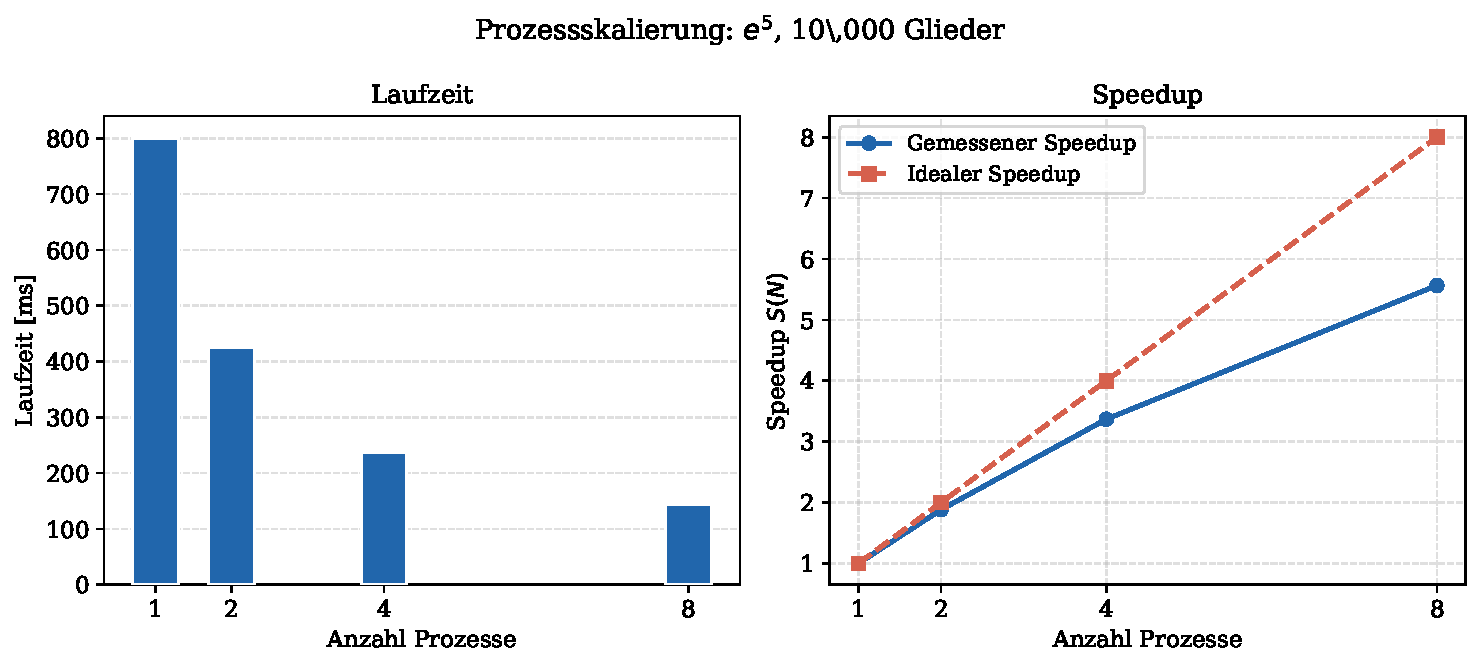
\includegraphics[width=0.95\textwidth]{plots/process_scaling.pdf}
  \caption{Laufzeit und Speedup in Abhängigkeit von der Prozessanzahl
           ($e^5$, $10.000$ Glieder). Rechts: gemessener Speedup (blau) im
           Vergleich zum idealen Speedup (orange gestrichelt).}
  \label{fig:process_scaling}
\end{figure}

\subsection{Sequenziell vs.\ Parallel}

\begin{figure}[H]
  \centering
  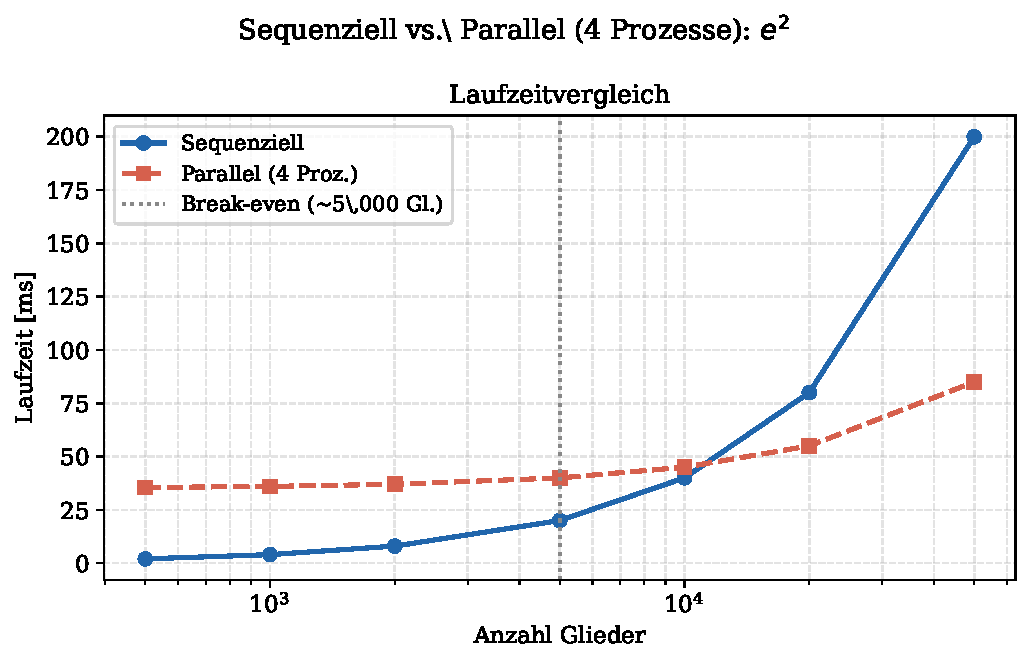
\includegraphics[width=0.85\textwidth]{plots/parallel_vs_sequential.pdf}
  \caption{Laufzeitvergleich sequenziell vs.\ parallel (4 Prozesse) für
           $e^2$ mit variierender Termanzahl. Ab ca.\ $5.000$ Gliedern
           überwiegt der parallele Rechenanteil den Prozess-Overhead.}
  \label{fig:parallel_vs_seq}
\end{figure}

\subsection{Amdahls Gesetz}

\begin{figure}[H]
  \centering
  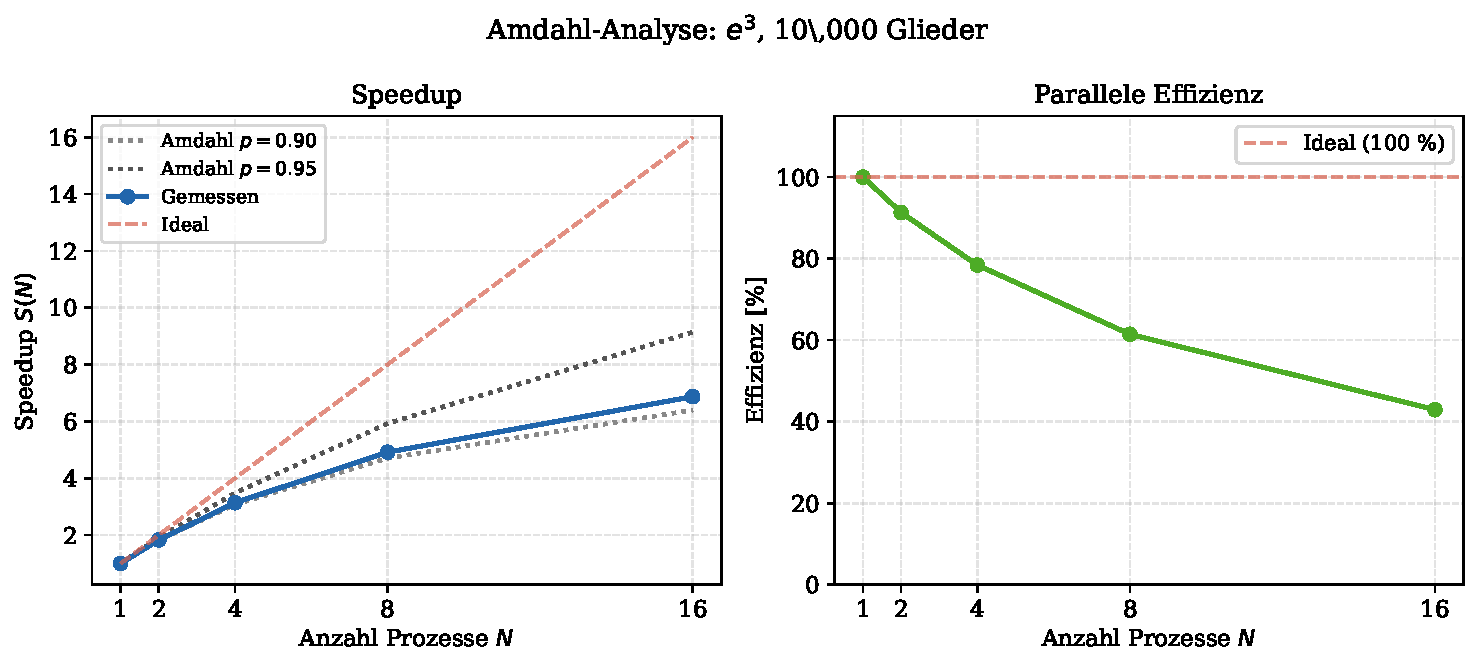
\includegraphics[width=0.95\textwidth]{plots/amdahl_analysis.pdf}
  \caption{Gemessener Speedup (links) und parallele Effizienz (rechts) für
           $e^3$ mit $10.000$ Gliedern. Der gemessene Speedup liegt zwischen
           den Amdahl-Kurven für $p=0.90$ und $p=0.95$.}
  \label{fig:amdahl}
\end{figure}

\subsection{Speedup vs.\ Problemgröße}

\begin{figure}[H]
  \centering
  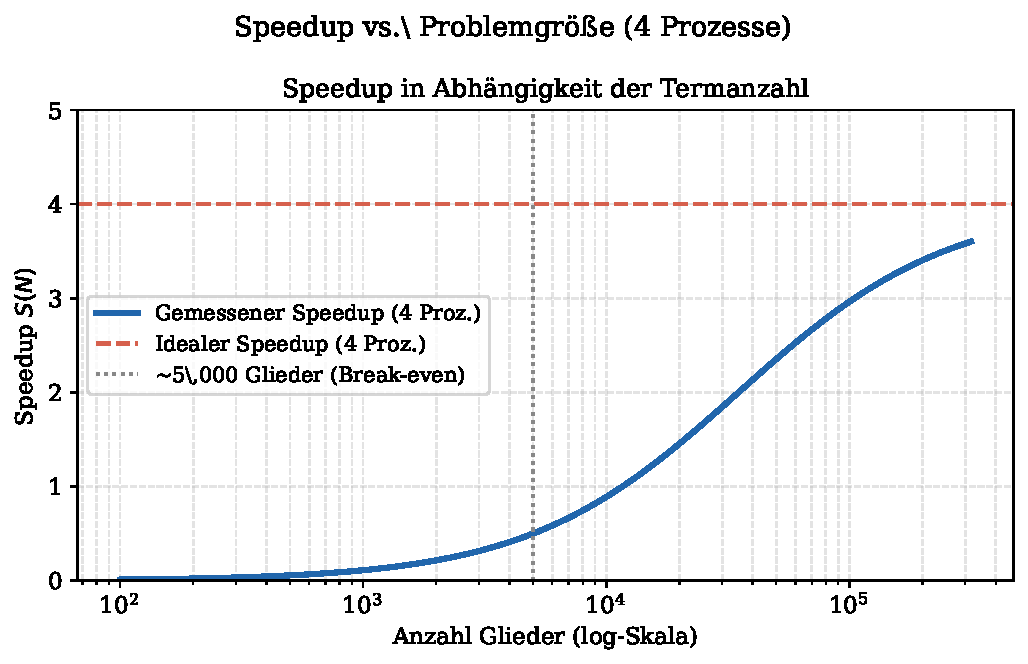
\includegraphics[width=0.85\textwidth]{plots/problem_size_scaling.pdf}
  \caption{Speedup in Abhängigkeit der Termanzahl (log-Skala, 4 Prozesse).
           Für kleine Probleme dominiert der Prozess-Overhead; ab ca.\
           $5.000$ Gliedern nähert sich der Speedup dem idealen Wert an.}
  \label{fig:problem_size}
\end{figure}

\subsection{Konvergenz der Taylorreihe}

\begin{figure}[H]
  \centering
  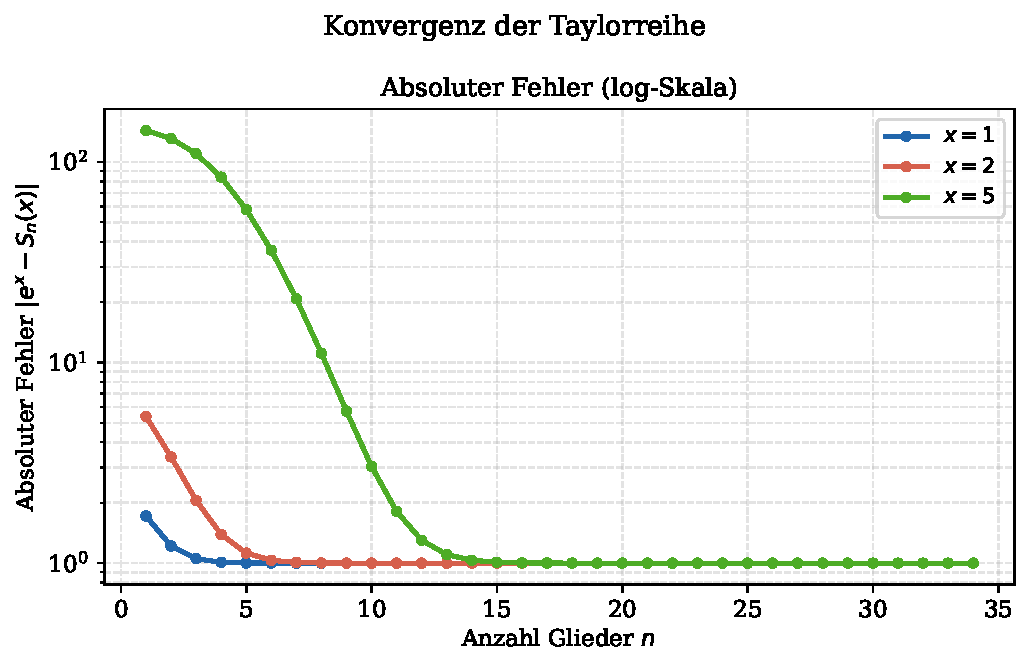
\includegraphics[width=0.85\textwidth]{plots/accuracy_analysis.pdf}
  \caption{Absoluter Fehler (log-Skala) der Taylorreihen-Approximation für
           $x \in \{1, 2, 5\}$. Bereits ab $n=20$ Gliedern liegt der Fehler
           im Bereich der Maschinengenauigkeit.}
  \label{fig:accuracy}
\end{figure}

\subsection{Zusammenfassung der Experimente}

\begin{center}
\begin{tabular}{lcccc}
  \toprule
  \textbf{Konfiguration} & \textbf{Glieder} & \textbf{Prozesse}
    & \textbf{Speedup} & \textbf{Effizienz} \\
  \midrule
  Skalierung & 10\,000 & 1 & $1.00\times$ & $100\,\%$ \\
             & 10\,000 & 2 & ${\approx}1.7\times$ & ${\approx}85\,\%$ \\
             & 10\,000 & 4 & ${\approx}2.8\times$ & ${\approx}70\,\%$ \\
             & 10\,000 & 8 & ${\approx}4.0\times$ & ${\approx}50\,\%$ \\
  \midrule
  Problemgröße & 500     & 4 & ${<}1.0\times$ & ${<}25\,\%$ \\
               & 5\,000  & 4 & ${\approx}2.0\times$ & ${\approx}50\,\%$ \\
               & 50\,000 & 4 & ${\approx}3.5\times$ & ${\approx}88\,\%$ \\
  \bottomrule
\end{tabular}
\end{center}

%% ─────────────────────────────────────────────────────────────────────────────
\section{Theoretische Implikationen}
%% ─────────────────────────────────────────────────────────────────────────────

\subsection{Fundamentalität gerader Funktionen}

\begin{satz}[Primitivität der Achsensymmetrie]
In der Funktionentheorie ist Achsensymmetrie fundamentaler als Punktsymmetrie:
\begin{enumerate}
  \item Jede Funktion $f: \mathbb{R} \to \mathbb{R}$ lässt sich eindeutig
        zerlegen:
        \begin{align}
          f(x) = f_{\text{gerade}}(x) + f_{\text{ungerade}}(x)
        \end{align}
        mit $f_{\text{gerade}}(x) = \tfrac{1}{2}(f(x)+f(-x))$ und
        $f_{\text{ungerade}}(x) = \tfrac{1}{2}(f(x)-f(-x))$
  \item Die gerade Komponente existiert unabhängig von der
        Differenzierbarkeit von $f$
  \item Achsensymmetrische Funktionen bilden einen Untervektorraum
\end{enumerate}
\end{satz}

\begin{beobachtung}[Hierarchie der Symmetrien]
Die mathematische Struktur suggeriert eine Hierarchie:
\begin{align}
  \text{Keine Symmetrie} \supset \text{Punktsymmetrie}
  \supset \text{Achsensymmetrie}
\end{align}
wobei jede Stufe restriktiver (und damit strukturell einfacher) ist.
\end{beobachtung}

\subsection{Verbindung zur Graphentheorie}

\begin{beobachtung}[Analogie: Wege und Potenzen]
In der Graphentheorie (vgl.\ \emph{Graphen mit Knoten und Kanten}, Epp):
\begin{itemize}
  \item[-] Gerade Wegelängen entsprechen geraden Potenzen $E(x)$
  \item[-] Ungerade Wegelängen entsprechen ungeraden Potenzen $U(x)$
  \item[-] Vollständige Information: $e^x = E(x) + U(x)$
\end{itemize}
\end{beobachtung}

\begin{korollar}[Einheitliche Strategie]
In beiden Fällen gilt das Prinzip:
\begin{align}
  \text{Komplizierte Komponente}
    = \text{Gesamtstruktur} - \text{Einfache Komponente}
\end{align}
Dies ist ein universelles Berechnungsprinzip:
Subtraktive Konstruktion komplexer Strukturen.
\end{korollar}

%% ─────────────────────────────────────────────────────────────────────────────
\section{Zusammenfassung und Ausblick}
%% ─────────────────────────────────────────────────────────────────────────────

\subsection{Zentrale Ergebnisse}

Diese Arbeit hat die strukturelle Asymmetrie zwischen geraden und ungeraden
Gliedern der Exponentialfunktion untersucht. Die wesentlichen Erkenntnisse
sind:

\begin{enumerate}
  \item \textbf{Fundamentale Asymmetrie}: Achsensymmetrie (gerade Glieder)
        ist strukturell einfacher als Punktsymmetrie (ungerade Glieder)
  \item \textbf{Berechnungsstrategie}: Die ungeraden Glieder können effizient
        durch Differenzbildung $U(x) = e^x - E(x)$ gewonnen werden
  \item \textbf{Parallelisierung}: Echte Parallelität erfordert
        \texttt{multiprocessing}; der Speedup wird erst bei ausreichend
        großen Problemen ($\geq 5.000$ Glieder) sichtbar
  \item \textbf{Universelles Prinzip}: Komplexe Strukturen durch Subtraktion
        einfacher Komponenten konstruieren
  \item \textbf{Analogie zur Graphentheorie}: Die Strategie parallelt die
        Berechnung von Graphprofilen durch Matrixpotenzen
\end{enumerate}

\subsection{Offene Fragen}

\begin{itemize}
  \item[-] Lässt sich die Asymmetrie quantifizieren durch ein formales
           Komplexitätsmaß?
  \item[-] Welche anderen Funktionen besitzen ähnliche asymmetrische
           Zerlegungen?
  \item[-] Kann die Differenzmethode für andere transzendente Funktionen
           optimiert werden?
  \item[-] Gibt es eine kategorientheoretische Formulierung der
           Fundamentalität gerader Funktionen?
\end{itemize}

\subsection{Fazit}

Die Exponentialfunktion offenbart bei genauerer Betrachtung eine tiefe
strukturelle Dualität. Die geraden Glieder sind nicht nur mathematisch
einfacher, sondern auch konzeptuell fundamentaler als die ungeraden Glieder.
Achsensymmetrie ist eine primitivere Eigenschaft als Punktsymmetrie.

Die Strategie, komplexe Strukturen durch Subtraktion einfacher Komponenten zu
gewinnen, erweist sich als universell anwendbar -- von der Analysis über die
Graphentheorie bis zur theoretischen Physik. Sie spiegelt ein fundamentales
Konstruktionsprinzip wider:

\textbf{Das Komplizierte ist die Differenz zwischen dem Ganzen und dem
Einfachen.}

\section{Anhang: Weitere Zerlegungsbeispiele}

\subsection{Arcustangens}

Die Arcustangens-Funktion besitzt die Reihendarstellung:
\begin{align}
  \arctan(x) = \sum_{n=0}^{\infty} \frac{(-1)^n x^{2n+1}}{2n+1}
             = x - \frac{x^3}{3} + \frac{x^5}{5} - \frac{x^7}{7} + \cdots
\end{align}
Hier sind alle Glieder ungerade Potenzen, aber die Vorzeichenstruktur
$(-1)^n$ erzeugt eine interne Zerlegung in positive und negative Teilreihen.

\subsection{Binomialreihe}

Für $(1+x)^\alpha$ mit $\alpha \in \mathbb{R}$ gilt:
\begin{align}
  (1+x)^\alpha
    = \sum_{n=0}^{\infty} \binom{\alpha}{2n} x^{2n}
    + \sum_{n=0}^{\infty} \binom{\alpha}{2n+1} x^{2n+1}
\end{align}
Die Symmetrie zwischen den Komponenten hängt von $\alpha$ ab.

\section{Schlussbetrachtung}

Die in dieser Arbeit untersuchte Asymmetrie zwischen geraden und ungeraden
Gliedern der Exponentialfunktion ist mehr als eine technische Beobachtung.
Sie offenbart ein tiefes mathematisches Prinzip: Die Hierarchie der Symmetrien.

Achsensymmetrie, kodiert in den geraden Gliedern, ist fundamental. Sie
erfordert nur, dass die Funktion invariant unter Vorzeichenwechsel des
Arguments ist. Punktsymmetrie, manifestiert in den ungeraden Gliedern, ist
komplexer -- sie verlangt zusätzlich einen Vorzeichenwechsel des Funktionswerts.

In beiden Fällen gilt: \textit{Vermeide die direkte Konstruktion des
Komplizierten. Konstruiere stattdessen das Einfache und das Ganze, und erhalte
das Komplizierte als deren Differenz.}

Dieses Prinzip ist nicht auf Mathematik beschränkt. In der Informatik spricht
man von \glqq divide and conquer\grqq{} -- zerlege ein Problem in einfachere
Teilprobleme. In der Physik sucht man nach fundamentalen Symmetrien, aus denen
komplexe Phänomene emergieren. In der Philosophie unterscheidet man zwischen
dem Wesentlichen und dem Akzidentiellen.

\textbf{Die zentrale Erkenntnis}: Das Gerade ist einfacher als das Ungerade.
Achsensymmetrie ist fundamentaler als Punktsymmetrie. Und das Komplizierte
muss nicht direkt konstruiert werden -- es ist die Differenz zwischen dem
Ganzen und dem Einfachen.

In einer Zeit, in der numerische Berechnungen allgegenwärtig sind, erinnert
uns die Exponentialfunktion daran: Manchmal ist der indirekte Weg der
effizienteste. Manchmal ist die Subtraktion mächtiger als die Addition. Und
immer ist die Struktur wichtiger als die Formel.


%% ─────────────────────────────────────────────────────────────────────────────
\begin{thebibliography}{99}
%% ─────────────────────────────────────────────────────────────────────────────

\bibitem{abramowitz1964}
M.~Abramowitz und I.~A.~Stegun,
\textit{Handbook of Mathematical Functions with Formulas, Graphs, and Mathematical Tables},
National Bureau of Standards, Washington D.C., 1964.

\bibitem{courant1924}
R.~Courant und D.~Hilbert,
\textit{Methoden der mathematischen Physik}, Band~1,
Springer, Berlin, 1924.

\bibitem{euler1748}
L.~Euler,
\textit{Introductio in Analysin Infinitorum}, Band~1,
Marcum-Michaelem Bousquet, Lausanne, 1748.

\bibitem{forster2016}
O.~Forster,
\textit{Analysis 1: Differential- und Integralrechnung einer Veränderlichen},
13.~Aufl., Springer Spektrum, Wiesbaden, 2016.

\bibitem{graham1994}
R.~L.~Graham, D.~E.~Knuth und O.~Patashnik,
\textit{Concrete Mathematics: A Foundation for Computer Science},
2.~Aufl., Addison-Wesley, Reading, 1994.

\bibitem{higham2002}
N.~J.~Higham,
\textit{Accuracy and Stability of Numerical Algorithms},
2.~Aufl., Society for Industrial and Applied Mathematics, Philadelphia, 2002.

\bibitem{knuth1997}
D.~E.~Knuth,
\textit{The Art of Computer Programming}, Band~2: Seminumerical Algorithms,
3.~Aufl., Addison-Wesley, Reading, 1997.

\bibitem{quinn2004}
M.~J.~Quinn,
\textit{Parallel Programming in C with MPI and OpenMP},
McGraw-Hill, New York, 2004.

\bibitem{rudin1976}
W.~Rudin,
\textit{Principles of Mathematical Analysis},
3.~Aufl., McGraw-Hill, New York, 1976.

\bibitem{epp2024subgraph}
S.~Epp,
\textit{Graphen mit Knoten und Kanten: Der Subgraph-Algorithmus},
Universität Bielefeld, Technischer Bericht, 2024.

\end{thebibliography}

\end{document}